\documentclass[hidelinks]{article}
\usepackage[ngerman]{babel} 
\usepackage[utf8x]{inputenc}
%% Hyperlinks 
\usepackage{hyperref}
\hypersetup{
    colorlinks,
    linkcolor={red!50!black},
    citecolor={blue!50!black},
    linktoc=all,
    urlcolor={blue!80!black}
}
%% Graphics
\usepackage{graphicx}
\usepackage{float}

\usepackage{enumerate}
% Math packages
\usepackage{amsmath}
\usepackage{amssymb}

% Algorithms
\usepackage{algorithm}
\usepackage[noend]{algpseudocode}
\newcommand\Let[2]{\State #1 $\gets$ #2}
\algrenewcomment[1]{\(\qquad \triangleright\) #1}
\newcommand\Blet[2]{\State \textbf{let} #1 \textbf{be} #2}
\errorcontextlines\maxdimen
% begin vertical rule patch for algorithmicx
% borrowing from http://tex.stackexchange.com/questions/41956/marking-conditional-versions-with-line-in-margin
% see http://tex.stackexchange.com/questions/110431/ploblems-with-vertical-lines-in-algorithmicx
\RequirePackage{zref-abspage}
\RequirePackage{zref-user}
\RequirePackage{tikz}
\RequirePackage{atbegshi}
\usetikzlibrary{calc}
\RequirePackage{tikzpagenodes}
\RequirePackage{etoolbox}
\makeatletter
\newcommand*\ALG@lastblockb{b}
\newcommand*\ALG@lastblocke{e}
\apptocmd{\ALG@beginblock}{%
    %\typeout{beginning block, nesting level \theALG@nested, line \arabic{ALG@line}}%
    \ifx\ALG@lastblock\ALG@lastblockb
        \ifnum\theALG@nested>1\relax\expandafter\@firstoftwo\else\expandafter\@secondoftwo\fi{\ALG@tikzborder}{}%
    \fi
    \let\ALG@lastblock\ALG@lastblockb%
}{}{\errmessage{failed to patch}}

\pretocmd{\ALG@endblock}{%
    %\typeout{ending block, nesting level \theALG@nested, line \arabic{ALG@line}}%
    \ifx\ALG@lastblock\ALG@lastblocke
        \addtocounter{ALG@nested}{1}%
        \addtolength\ALG@tlm{\csname ALG@ind@\theALG@nested\endcsname}%
        \ifnum\theALG@nested>1\relax\expandafter\@firstoftwo\else\expandafter\@secondoftwo\fi{\endALG@tikzborder}{}%
        \addtolength\ALG@tlm{-\csname ALG@ind@\theALG@nested\endcsname}%
        \addtocounter{ALG@nested}{-1}%
    \fi
    \let\ALG@lastblock\ALG@lastblocke%
}{}{\errmessage{failed to patch}}
\tikzset{ALG@tikzborder/.style={line width=0.5pt,black}}
\newcommand*\currenttextarea{current page text area}
\newcommand*{\updatecurrenttextarea}{%
    \if@twocolumn
        \if@firstcolumn
            \renewcommand*{\currenttextarea}{current page column 1 area}%
        \else
            \renewcommand*{\currenttextarea}{current page column 2 area}%
        \fi
    \else
        \renewcommand*\currenttextarea{current page text area}%
    \fi
}
\newcounter{ALG@tikzborder}
\newcounter{ALG@totaltikzborder}
\newenvironment{ALG@tikzborder}[1][]{%
    % Allow user to overwrite the used style locally
    \ifx&#1&\else
        \tikzset{ALG@tikzborder/.style={#1}}%
    \fi
    \stepcounter{ALG@totaltikzborder}%
    \expandafter\edef\csname ALG@ind@border@\theALG@nested\endcsname{\theALG@totaltikzborder}%
    \setcounter{ALG@tikzborder}{\csname ALG@ind@border@\theALG@nested\endcsname}%
    %\typeout{begin ALG border nesting level=\theALG@nested, tikzborder=\theALG@tikzborder, tlm=\the\ALG@tlm}%
    \tikz[overlay,remember picture] \coordinate (ALG@tikzborder-\theALG@tikzborder);% node {\theALG@tikzborder};% Modified \tikzmark macro
    \zlabel{ALG@tikzborder-begin-\theALG@tikzborder}%
    % Test if end-label is at the same page and draw first half of border if not, from start place to the end of the page
    \ifnum\zref@extract{ALG@tikzborder-begin-\theALG@tikzborder}{abspage}=\zref@extract{ALG@tikzborder-end-\theALG@tikzborder}{abspage} \else
        \updatecurrenttextarea
        \ALG@drawvline{[shift={(0pt,.5\ht\strutbox)}]ALG@tikzborder-\theALG@tikzborder}{\currenttextarea.south east}{\ALG@thistlm}%
        % If it spreads over more than two pages:
        \newcounter{ALG@tikzborderpages\theALG@tikzborder}%
        \setcounter{ALG@tikzborderpages\theALG@tikzborder}{\numexpr-\zref@extract{ALG@tikzborder-begin-\theALG@tikzborder}{abspage}+\zref@extract{ALG@tikzborder-end-\theALG@tikzborder}{abspage}}%
        \ifnum\value{ALG@tikzborderpages\theALG@tikzborder}>1
            \edef\nextcmd{\noexpand\AtBeginShipoutNext{\noexpand\ALG@tikzborderpage{\theALG@tikzborder}{\the\ALG@thistlm}}}%some pages need a border on the whole page
            \nextcmd
        \fi
    \fi
}{%
    \setcounter{ALG@tikzborder}{\csname ALG@ind@border@\theALG@nested\endcsname}%
    %\typeout{end ALG border nesting level=\theALG@nested, tikzborder=\theALG@tikzborder, tlm=\the\ALG@tlm}%
    \tikz[overlay,remember picture] \coordinate (ALG@tikzborder-end-\theALG@tikzborder);% node {\theALG@tikzborder};% Modified \tikzmark macro
    \zlabel{ALG@tikzborder-end-\theALG@tikzborder}%
    % Test if begin-label is at the same page and draw whole border if so, from start place to end place
    \updatecurrenttextarea
    \ifnum\zref@extract{ALG@tikzborder-begin-\theALG@tikzborder}{abspage}=\zref@extract{ALG@tikzborder-end-\theALG@tikzborder}{abspage}\relax
        \ALG@drawvline{[shift={(0pt,.5\ht\strutbox)}]ALG@tikzborder-\theALG@tikzborder}{ALG@tikzborder-end-\theALG@tikzborder}{\ALG@thistlm}%
    % Otherwise draw second half of border, from the top of the page to the end place
    \else
        %\settextarea
        \ALG@drawvline{\currenttextarea.north west}{ALG@tikzborder-end-\theALG@tikzborder}{\ALG@thistlm}%
    \fi
}
\newcommand*{\ALG@drawvline}[3]{%#1=from, #2=to, #3=value of \ALG@tlm/\ALG@thisthm
    \begin{tikzpicture}[overlay,remember picture]
        \draw [ALG@tikzborder]
            let \p0 = (\currenttextarea.north west), \p1=(#1), \p2 = (#2)
             in
            (#3+\fboxsep+.5\pgflinewidth+\x0,\y1+\fboxsep+.5\pgflinewidth)%-\fboxsep-.5\pgflinewidth
             --
            (#3+\fboxsep+.5\pgflinewidth+\x0,\y2-\fboxsep-.5\pgflinewidth)
            %node[midway,anchor=east] {\ALG@tikzbordertext}
        ;
    \end{tikzpicture}%
}
\newcommand{\ALG@tikzborderpage}[2]{%the whole page gets a border, #1=value of \theALG@tikzborder, #2=value of \ALG@tlm/\ALG@thistlm
    \updatecurrenttextarea
    \setcounter{ALG@tikzborder}{#1}%
    \ALG@drawvline{\currenttextarea.north west}{\currenttextarea.south east}{#2}%
    \addtocounter{ALG@tikzborderpages\theALG@tikzborder}{-1}%
    \ifnum\value{ALG@tikzborderpages\theALG@tikzborder}>1
        \AtBeginShipoutNext{\ALG@tikzborderpage{#1}{#2}}%
    \fi
    \vspace{-0.5\baselineskip}% Compensate for the generated extra space at begin of the page. No idea why exactly this happens.
}
\def\ALG@tikzbordertext{\the\ALG@tlm}
\makeatother
% end vertical rule patch for algorithmicx

% continuation indent patch, slightly extended from http://tex.stackexchange.com/questions/78776/forced-indentation-in-algorithmicx to support multiple paragraphs in one block
\RequirePackage{etoolbox}
\makeatletter
\newlength{\ALG@continueindent}
\setlength{\ALG@continueindent}{2em}
\newcommand*{\ALG@customparshape}{\parshape 2 \leftmargin \linewidth \dimexpr\ALG@tlm+\ALG@continueindent\relax \dimexpr\linewidth+\leftmargin-\ALG@tlm-\ALG@continueindent\relax}
\newcommand*{\ALG@customparshapex}{\parshape 1 \dimexpr\ALG@tlm+\ALG@continueindent\relax \dimexpr\linewidth+\leftmargin-\ALG@tlm-\ALG@continueindent\relax}
\apptocmd{\ALG@beginblock}{\ALG@customparshape\everypar{\ALG@customparshapex}}{}{\errmessage{failed to patch}}
\makeatother
% end continuation indent patch
\usepackage{mathtools}

% Proof system
\usepackage{amsthm}
\theoremstyle{plain}
\newtheorem{thm}{Theorem}[section]
\newtheorem{lem}[thm]{Lemma}
\newtheorem{prop}[thm]{Proposition}
\theoremstyle{definition}
\newtheorem{defn}[thm]{Definition}
\newtheorem{bsp}[thm]{Example}
\newtheoremstyle{rem} % name
    {\topsep}                    % Space above
    {\topsep}                    % Space below
    {}                   % Body font
    {}                           % Indent amount
    {\bf}                   % Theorem head font
    {:}                          % Punctuation after theorem head
    {.5em}                       % Space after theorem head
    {}  % Theorem head spec (can be left empty, meaning ‘normal’)
\theoremstyle{rem}
\newtheorem*{remark}{Note}
%\usepackage{xpatch}
%\makeatletter
%% Remove last point from definitions, theorems, etc.
%\xpatchcmd{\@thm}{\thm@headpunct{.}}{\thm@headpunct{\\}}{}{}
%\makeatother

% Seitenränder
%originally 1.5 in
\usepackage[margin=1in]{geometry}
\usepackage{wrapfig}
% citations
\usepackage{cite}
% Graphs
\usepackage{tikz}
\usetikzlibrary{calc,arrows.meta,positioning}
\usepackage{tikz-3dplot}
\usepackage{subfig}
\usepackage{pgfplots}
\pgfplotsset{%
    ,compat=1.12
    ,every axis x label/.style={at={(current axis.right of origin)},anchor=north west}
    ,every axis y label/.style={at={(current axis.above origin)},anchor=north east}
    }
\setlength{\parindent}{0pt}

% Custom commands
\newcommand{\fromto}[2]{\{#1,\ldots,#2\}}

\pagestyle{plain}

%------------------------------------------------------------------------------
\begin{document}

\pagenumbering{arabic}

\begin{sloppypar}
\begingroup  
  \LARGE Einführung in die Informatik 2 - Repetitorium WS 2016/17\\Technische Universität München\\[0.5em]
  \large{Kevin Kappelmann\hfill \today}\\
\endgroup
\hrule height 1pt
{\LARGE{{\begin{center}\textbf{Induktion - Prinzip und Fallbeispiel}\end{center}}}}
\section{Theorie}
Induktion ist einer der wichtigsten Beweismittel eines Informatikers. Es ist äußerst wichtig, nicht nur Induktionen durchführen zu können, sondern vor allem auch ihr Prinzip und ihre Struktur zu verstehen.\\
Induktionen können ganz allgemein über partielle Ordnungen, die keine unendlich absteigenden Ketten besitzen, durchgeführt werden. Oft verwenden wir als Universum der partiellen Ordnung $\mathbb{N}_0$ und als partielle Ordnung die ``Kleiner-Gleich-Relation'' $\le\subset\mathbb{N}_0\times\mathbb{N}_0$. Besitzen wir also nun eine solche partielle Ordnung $\preceq\subseteq M\times M$ und wollen die Gültigkeit von $P(m)$ für alle Elemente $m$ unseres Universums M zeigen, so können wir wie folgt verkehren:
\begin{enumerate}
\item Zeige die Gültigkeit von P(b) für alle $b\in M$, die keine Vorgänger bezüglich $\preceq$ besitzen (diese existieren, da $\preceq$ keine unendlich absteigende Ketten besitzt).
\item Fixiere ein beliebiges $m\in M$, welches Vorgänger $v_0,v_1,\ldots,v_n$ bezüglich $\preceq$ besitzt.
\begin{enumerate}
\item Nimm an, es gelte $P(v_0),\ldots,P(v_n)$
\item Zeige, dass dann auch $P(m)$ gilt.
\end{enumerate}
\end{enumerate}
\section{Fallbeispiele}
Wem das jetzt alles etwas zu abstrakt war, der darf sich jetzt auf zwei angewandte Beispiele freuen, in dem das Ganze hoffentlich klarer wird.
\subsection{Gauß das Wunderkind}
Von 1777 bis 1855 lebte einst einer der einflussreichsten Mathematiker aller Zeiten Carl Friedrich Gauß. Damals schon als ``Princeps Mathematicorum'' bezeichnet, was so viel wie ``Fürst der Mathematik'' heißt, entdeckte er bereits als 9-jähriger Schüler, als er als Aufgabe die Summe der Zahlen $1,2,\ldots,n$ ausrechnen musste, die gaußsche Summenformel
\begin{equation}
\sum_{i=0}^{n}i=\frac{n*(n+1)}{2},\forall n\in \mathbb{N}_0\label{gauss_sum}
\end{equation}
Auch wenn der neunjährige Gauß diese damals wohl nicht mit Induktion bewies, wollen wir dies nun tun.
\begin{wrapfigure}{r}{0.25\textwidth}
	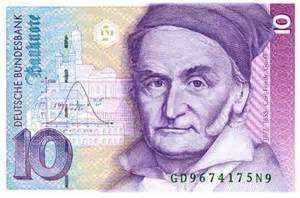
\includegraphics[width=4.5cm]{gauss.jpg}
	\centering
	\caption*{\small{Gauß war übrigens auf dem 10DM-Schein und schaut euch bei eurer EIDI2-Klausur von oben zu ;)}}
\end{wrapfigure}
\begin{prop}
Für alle $n\in \mathbb{N}_0$ gilt die gaußsche Summenformel~\eqref{gauss_sum}
\end{prop}
\begin{proof}
Wir zeigen die Aussage mit Induktion über n.
\begin{itemize}
\item \underline{Induktionsbasis:} Sei n=0, dann
\begin{equation*}
	\sum_{i=0}^{0}i=0=\frac{0*(0+1)}{2}
\end{equation*}
\item \underline{Induktionsschritt:} Sei $n\in \mathbb{N}_0$ beliebig fixiert
	\begin{itemize}
	\item \underline{Induktionshypothese:} Es gelte $\sum_{i=0}^{n}i=\frac{n*(n+1)}{2}$
	\item \underline{Induktionsbehauptung:} Dann gilt auch $\sum_{i=0}^{n+1}i=\frac{(n+1)*((n+1)+1)}{2}$
	\item \underline{Beweis:}
	\begin{align*}
		\sum_{i=0}^{n+1}i&=n+1+\sum_{i=0}^{n}i\stackrel{I.H.}{=}n+1+\frac{n*(n+1)}{2}=n+1+\frac{n^2+n}{2}=\frac{2n+2+n^2+n}{2}\\
		&=\frac{(n^2+2n+1)+n+1}{2}=\frac{(n+1)^2+n+1}{2}=\frac{(n+1)*((n+1)+1)}{2}
	\end{align*}
	\end{itemize}
\end{itemize}
\hfill
\end{proof}
\textbf{Bitte schreibt eure Induktionsbeweise stets so strukturiert, wie in diesem Beispiel! Behaltet am besten einfach diese Form bei.}
\subsection{Eine Basis ist nicht genug}
Der folgende Fall ist (wahrscheinlich) für EIDI2 nicht interessant, nichtsdestotrotz wollen wir ihn hier kurz besprechen.\\
Wir betrachten folgende Sequenz
\begin{equation}
a_1=1,\qquad a_2=8,\qquad a_{n+2}=a_{n+1}+2*a_n,\quad\forall n\in\mathbb{N}
\end{equation}
\begin{prop}
Für alle $n\in\mathbb{N}$ gilt
\begin{equation*}
	a_n=3*2^{n-1}+2(-1)^n\eqqcolon f(n)
\end{equation*}
\end{prop}
\begin{proof}
Wir zeigen die Aussage mit Induktion über n. Wir bemerken, dass die Definition von $a_{n+2}$ sowohl von $a_n$ als auch von $a_{n+1}$ abhängig ist, weswegen wir, um im Induktionsschritt die Induktionshypothese für zwei Vorgänger annehmen zu können, im Basisfall sowohl die Aussage für $n=1$ als auch für $n=2$ beweisen müssen.
\begin{itemize}
\item \underline{Induktionsbasis:} 
\begin{itemize}
\item \underline{$n=1$:}\qquad$a_1\stackrel{Def.}{=}1=3*2^0-2=f(1)$
\item \underline{$n=2$:}\qquad$a_2\stackrel{Def.}{=}8=3*2^1+2=f(2)$
\end{itemize}
\item \underline{Induktionsschritt:} Sei $n\in \mathbb{N}$ beliebig fixiert
	\begin{itemize}
	\item \underline{Induktionshypothese:} Es gelte $a_n=f(n)$ und $a_{n+1}=f(n+1)$
	\item \underline{Induktionsbehauptung:} Dann gilt auch $a_{n+2}=f(n+2)$
	\item \underline{Beweis:}
	\begin{align*}
		a_{n+2}&\stackrel{Def.}{=}a_{n+1}+2*a_n\stackrel{I.H.}{=}3*2^n+2*(-1)^{n+1}+2*(3*2^{n-1}+2*(-1)^n)\\
		&=2*3*2^n+2*((-1)^{n+1}+2*(-1)^n)\\
		&=3*2^{n+1}+2*((-1)^n*(-1+2))=3*2^{n+1}+2*(-1)^n\\
		&=3*2^{n+1}+2*(-1)^{n+2}
	\end{align*}
	\end{itemize}
\end{itemize}
\hfill
\end{proof}

\section{Übungen}
\begin{itemize}
\item Ein kleiner Gauß ist zu wenig! Zeigen Sie: $\sum_{i=0}^{n}i^2=\frac{n*(n+1)(2*n+1)}{6}$
\item DS-Flashbacks: Die Anzahl der Holztüren Eiche fundiert mit Plastikgriff (kurz: HtEfmPg) der Preisklasse n ist durch folgende Funktion definiert
\begin{equation}
HtEfmPg(n)\coloneqq\begin{cases}
		1, & \text{falls $n=1$}\\
		2, & \text{falls $n=2$}\\
	   	2*HtEfmPg(n+1)-HtEfmPg(n)+1, & \text{sonst}
	\end{cases}
\end{equation}
Zeigen Sie: $HtEfmPg(n)=0.5*(n^2+n+2)$
\end{itemize}
\end{sloppypar}
\end{document}
